\section{Software}
This section describs the software used in this master thesis.
Lucene were used in the initial implementation of query expansion.
The last experiment utilized Node.JS as the webserver and Elasticsearch as the search engine.

\subsection{Node.js}
Node.js\footnote{\url{https://nodejs.org}} version 7 was chosen as the webserver.
Node.js was chosen because the author has knowledge of the technology,
and it contains a rich package manager called NPM.
By utilizing open source libraries through NPM, more time could be spent implementing the algoritms for query expansion.
Inside NodeJS lies the V8\footnote{\url{https://developers.google.com/v8/}} JavaScript engine.

\subsection{Lucene}
Lucene\footnote{\url{https://lucene.apache.org/}} is an open-source full-text search engine library written in Java.
According to Lucene\footnote{\url{http://lucene.apache.org/core/}} the index size is only about 20-30\% of the original text.
Lucene's search features features such as ranked search, field search and faceting, to mention a few.

Lucene exposes the low level API's which gives very much control over the inner workings of Lucene.
Table \ref{tbl:inverted-index} shows a low level data structure inside Lucene called an inverted index.
The table contains a list of all the possible terms inside a text.
The second column is the frequency each term has.
Lastly, the documents column list all the documents where the given term occurs.
An inverted index requires more resources when indexing,
but the data structure are effective when searching.
The query expansion which is used in this master thesis requires information stored in the inverted index.

To illustrate how the inverted index works, Lucene recieves a query for the terms \texttt{blue}.
Using table \ref{tbl:inverted-index} the inverted index shows that the term has a frequency of three,
and that the term occurs in document 1, 2 and 3.
A search result would then return document 1, 2 and 3.

One important drawback with Lucene is that it is not scalable across multiple machines.
However, scalable across multiple machines are on of the advantages of using Elasticsearch.

\begin{table}[h]
    \centering
    \begin{tabular}{l|l|l}
    Term   & Frequency & Documents                                                 \\ \hline
    blue   & 3         & Document 1, document 2, document 3                        \\
    sky    & 1         & Document 2                                                \\
    clouds & 4         & Document 2, document 3, document 4, document 5            \\
    rain   & 2         & Document 2, document 5                                    \\
    plane  & 2         & Document 1, document 4                                    \\
    sunset & 5         & Document 1, document 2, document 3, document 4 document 5 \\
    \end{tabular}
    \caption{Example of an inverted index inside Lucene}
    \label{tbl:inverted-index}
\end{table}


\subsection{Elasticsearch}
Elasticsearch\footnote{\url{https://www.elastic.co/products/elasticsearch}} v5 were used as the search engine in the implementation described in this master thesis.
Elasticsearch has proven the ability to scale up to petabytes of data \cite{elasticsearch-scale}.
Elasticsearch is open source and built on top of Lucene.
Lucene is the search engine itself,
and Elasticsearch provides functionality for distribution and a REST API interface.

The following topics describes basic termonology used in Elasticsearch.
This information is needed to understand some of the results and observations,
and the implementation described in chapter \ref{ch:approach} and chapter \ref{ch:evaluation}.

\subsubsection{Cluster}
One or more servers connected together is called a cluster.
Elasticsearch indices are divided into shards which are distributed across the servers in the cluster.
Queries is also distributed to all the servers in the cluster, which again increases the performance.
Elasticsearch is responsible for distributing the shards across the physical servers,
and makes sure that replica shards are not on the same physical server.
The cluster used in this master thesis consisted of one server.

\subsubsection{Node Types}
Elasticsearch have four different node types: master node, data node, ingest node and tribe node.
The master node is responsible of handling administrative cluster tasks such as:
creating or deleting an index, tracking online and offline nodes and deciding how the shards should be distributed.
Data nodes is responsible for holding the shards and executing queries.
Ingest nodes is used as pre-processing nodes.
A tribe node is handling the coordination of querying and indexing.
Tribe nodes i also known as coordination nodes.
All nodes in a cluster is also an coordination node.


\subsubsection{Sharding}
The stored data in Elasticsearch may grow to become larger than the hardware on a single machine can handle,
both in size and in number of requests.
To mitigate the problem elasticsearch splits each index into multiple segments called shards.
Each of this shards may be distributed across multiple nodes.
This leads to higher performance when indexing new documents and when searching the documents.
The shards may also be duplicated to support higher query volumes and availability.

There is important distinction between an Elasticsearch index and a Lucene index.
A Lucene index, is the index which contains the inverted indices and holds all the data.
An Elasticsearch index on the other hand consists of on or more shards.
One Elasticsearch shard is the same as a Lucene index.

However, when the cluster consists of multiple nodes a query strategy is required.
Figure \ref{fig:elasticsearch-sharding} illustrates how an index may be distributed across three nodes.
The figure shows a simplified view on how a query are distributed across three nodes.
First the query arrives a coordination node.
The coordination node parses the query and determines which nodes holds shards for the given index.
Each shard determines locally which documents are most relevant from the query.
Metada from all the shards are then sent back to the coordination node.
On the coordination node alle the retrieved metadata are used to calculate the global result.
After the global result have been calculated,
all the shards are then queried for the documents from the global result.
After the documents are retrieved the result are returned back to the client.

\begin{figure}[h]
  \centering
  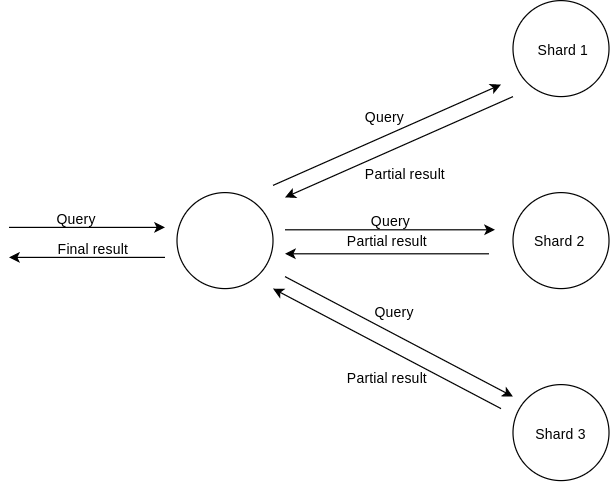
\includegraphics[width=0.9\linewidth]{img/elasticsearch-sharding.png}
  \caption{Elasticsearch distributing query agains all the shards}
  \label{fig:elasticsearch-sharding}
\end{figure}

\subsubsection{Aproximate Values}
As a result of Elasticsearch's distributed nature some queries will return estimated values.
Aggregations in Elasticsearch is an example which may return estimated values.

Table \ref{tbl:shard-term-counts} has a list of words across three different shards.
The term frequencies are listed inside the parenthesis.
When a client queries for the top three terms, the query is distributed to the shards.
Each shard then returns their local top three terms.
Given Table \ref{tbl:shard-term-counts},
the shards will return the terms listed in table \ref{tbl:shard-top}.
On the coordination node the global top three terms are calculated.
The top three terms is listed in table \ref{tbl:final-result}, which are \texttt{blue}, \texttt{sky} and \texttt{clouds}.
However, \texttt{blue}, \texttt{sky} and \texttt{clouds} are not the actual top three terms.
If the coordination node had all the knowledge in table \ref{tbl:shard-term-counts},
the top three terms would be \texttt{blue}, \texttt{sky} and \texttt{insta},
with the term frequencies 60, 32 and 22 respectively.
With global knowledge both the frequencies and one of the top 3 terms have changed.

The example explained above is exaggerated to illustrate what might happen in Elasticsearch's distributed architechture.
Even though the result is not exact, it is good enough for most use cases.
Elasticsearch can be configured to return more exact results,
at the cost of longer response times.

\begin{table}[h!]
    \centering
    \begin{tabular}{|l|c|c|c|}
    \hline
    ~ & \textbf{Shard 1}    & \textbf{Shard 2}     & \textbf{Shard 3}    \\ \hline
    1 & blue (10)  & blue (20)   & blue (30)  \\ \hline
    2 & clouds (9) & clouds (12) & sky (25)   \\ \hline
    3 & sky (5)    & insta (5)   & insta (15) \\ \hline
    4 & plane (4)  & plane (3)   & plane (10) \\ \hline
    5 & insta (2)  & sky (2)     & rain (3)   \\ \hline
    \end{tabular}
    \caption{Term list with the corresponding term count.}
    \label{tbl:shard-term-counts}
\end{table}

\begin{table}[h!]
    \centering
    \begin{tabular}{|l|c|c|c|}
    \hline
    ~ & \textbf{Shard 1}    & \textbf{Shard 2}     & \textbf{Shard 3}    \\ \hline
    1 & blue (10)  & blue (20)   & blue (30)  \\ \hline
    2 & clouds (9) & clouds (12) & sky (25)   \\ \hline
    3 & sky (5)    & insta (5)   & insta (15) \\ \hline
    \end{tabular}
    \caption{Term list of the top three terms returned to the coordination node.}
    \label{tbl:shard-top}
\end{table}

\begin{table}[h!]
    \centering
    \begin{tabular}{|l|c|}
    \hline
    ~ & \textbf{Returned result} \\ \hline
    1 & blue (60)     \\ \hline
    2 & sky (30)    \\ \hline
    3 & clouds (21)       \\ \hline
    \end{tabular}
    \caption{Top three terms which are returned back to the client.}
    \label{tbl:final-result}
\end{table}

https://www.elastic.co/guide/en/elasticsearch/reference/current/search-aggregations-bucket-terms-aggregation.html
